\documentclass[conference]{IEEEtran}
\usepackage{amsmath,amssymb,graphicx,booktabs,textcomp,url,cite}
\usepackage[T1]{fontenc}
\hyphenation{Sentinel DarkRS ExDark}
\begin{document}
\title{Training-Free Illumination-Aware Gamma Correction for Remote Sensing Imagery: A Multi-Dataset Benchmark with Integrity Controls}
\author{\IEEEauthorblockN{[Authors to be added]}\IEEEauthorblockA{Draft manuscript generated from \texttt{research/manuscript/first\_draft.md}}}
\maketitle
\begin{abstract}
We study how far a training-free, locally adaptive gamma correction can improve contrast in low-light and non-uniformly illuminated remote-sensing imagery while preserving structure and band ratios, and when terrain-derived illumination adds benefit. We freeze an existing method, TASC-Gamma (TASC-v0), in two configurations (image-only and DEM-assisted) and evaluate it against ten baselines (including per-band variants and shared-gain variants of histogram methods) and a set of benchmark-integrity controls on six datasets and a downstream probe: controlled Landsat pairs (6 source crops of one scene $\times$ 10 synthetic variants), Sentinel-2 L2A with Copernicus DEM (24 acquisitions, 6 regions, 2 held out), synthetically darkened AID (210 source images $\times$ 3 degradations) and iSAID-dark (46 parent images), real night imagery from DarkRS (86) and ExDark (400), and an AID scene-classification probe. Repeated variants or degradations of one source are averaged before testing. On the Landsat benchmark that TASC-v0 was designed on it has the highest PSNR of all baselines (21.65 dB versus 19.22 dB for global gamma and 16.89 dB for Zero-DCE), in all six crops, although no comparison is significant after Holm correction with n = 6; controls show that the DEM helps only when correctly registered, but those shadows are synthesised from the same DEM. Shared-gain methods preserve the input's band ratios by construction (corrected spectral angle to the input 0$^{\circ}$); this is preservation, not recovery of surface reflectance. A spectral-angle advantage of TASC over the input that we first reported on Sentinel-2 was an artefact of a defective metric and is withdrawn. On real Sentinel-2 terrain the DEM-assisted variant lifts DEM-derived shadow pixels more than the image-only variant (0.218 versus 0.193 on four development regions; exploratory, circular masks), but a material-matched equalisation proxy does not improve. Outside controlled terrain shading the image-only method performs poorly: on AID it is 4.1 dB below global gamma and 6.0 dB below the best baseline in PSNR, on iSAID-dark it is below the unprocessed input, it lowers entropy and gives worse BRISQUE than the input on real night images, and it reduces linear-probe classification accuracy by 15--24 percentage points. An ablation points to the global exposure step as the main cause. SAGC, SAMSIE and DFFN were not evaluated. We report all negative findings, the missing baselines, and the proxy nature of our terrain metrics.
\end{abstract}
\begin{IEEEkeywords}
low-light enhancement, gamma correction, remote sensing, digital elevation model, topographic shadow, benchmark.
\end{IEEEkeywords}
\section{Introduction}
Optical remote-sensing images are frequently under-exposed, either because they are acquired at night or in twilight, or because large parts of the scene lie in terrain shadow. Learned enhancement networks can brighten such images, but they need paired training data, can alter spectral relations, and are costly to run on large scenes. Classical histogram and gamma methods are cheap and training-free, but they operate globally or on small windows and typically treat each band independently, which distorts band ratios and indices such as NDVI.

TASC-Gamma (here frozen as TASC-v0) is a training-free pipeline that combines block-adaptive gamma with an optional terrain-derived shadow prior from a digital elevation model (DEM) and a single gain shared across bands, so that band ratios are unchanged. It was developed on Landsat data. This paper does not modify it. Instead it asks the research question: \emph{how far can training-free, locally adaptive gamma correction improve contrast in low-light or non-uniformly illuminated remote-sensing imagery while preserving structure and spectra, and when does terrain-derived illumination add benefit?}

Our contributions are an evaluation, not a new algorithm:

\begin{enumerate}
\item a multi-dataset benchmark protocol with a fixed a-priori split into development and held-out regions, region-level statistics and a coverage report;
\item benchmark-integrity controls (no DEM, constant-weight, wrong, flipped and shifted DEM, perturbed sun angles, global versus local gamma, with and without the DCT detail step, with and without the shared gain) that probe whether the DEM is genuinely used;
\item an honest account of where the frozen method works (controlled terrain shading, spectral preservation) and where it does not (synthetic and real low-light imagery, downstream classification); and
\item a list of what was not done: unavailable baselines, proxy metrics, and the limited number of independent regions.
\end{enumerate}
\section{Related Work}
\textbf{Histogram and gamma enhancement.} Contrast-limited adaptive histogram equalisation (CLAHE) \cite{zuiderveld1994clahe} equalises tiled histograms with clipping and bilinear blending. Adaptive gamma correction with weighting distribution (AGCWD) \cite{huang2013agcwd} derives a gamma curve from the smoothed histogram, and adaptive gamma correction (AGC) \cite{rahman2016agc} adapts the gamma to image statistics. These methods are applied to luminance or to each band, and do not use terrain information.

\textbf{Spatially adaptive gamma for remote sensing (SAGC, SAMSIE).} Spatially adaptive gamma correction is established prior art in remote-sensing enhancement and is not claimed as novel here. SAGC \cite{huang2018sagc} targets low-contrast optical remote-sensing images: per its abstract, it separates a base and a detail layer with relative total variation, applies an adaptive gamma correction to the base layer, and recombines the result with the corrected detail layer, with the aim of brightening while preserving weak structures. SAMSIE \cite{huang2022samsie}, by the same first author, is described as a spatially adaptive multi-scale scheme: a nonsubsampled contourlet transform splits the image into scales, an adaptive operator treats fine details, and the base layer is corrected by a spatially adaptive gamma correction built on improved histogram equalisation (SAGC-IHE). We read both from their published abstracts and bibliographic records; we did not obtain verified reference code for either, and therefore \textbf{did not evaluate SAGC or SAMSIE}. Our "2D-gamma" baseline is an independent, simplified spatially varying gamma and must not be read as a reproduction of either. To the extent that can be established from those abstracts, these methods adapt gamma from image content alone (no DEM or sun geometry) and do not state a mechanism that keeps inter-band ratios unchanged; whether they do so for multispectral input is not something we can assert. TASC-v0 shares their general idea of local gamma on a smoothed base layer and a separate detail step; the elements specific to TASC-v0 are the DEM-derived shadow prior and the single gain shared across bands. This paper evaluates TASC-v0 and makes no priority claim for the underlying ideas.

\textbf{Learned low-light enhancement.} Zero-DCE \cite{guo2020zerodce} estimates pixel-wise curve parameters without paired data, and we evaluate it with the official weights. DFFN \cite{yao2024dffn} is a learned spatial--frequency dual-domain feature-fusion network for low-light remote-sensing enhancement (amplitude and phase branches with an information-fusion affine block); its authors state that they built two low-light remote-sensing datasets and release code at \texttt{iijjlk/DFFN}, from whose README our iSAID-dark copy was obtained. We downloaded the DFFN weights but \textbf{did not run DFFN} (Section IX), so no DFFN result is reported; DFFN's published numbers are not comparable to ours.

\textbf{Topographic correction.} The C-correction \cite{teillet1982ccorr} and SCS+C \cite{soenen2005scsc} normalise illumination using the angle between the surface normal and the sun, computed from a DEM, and are usually applied to surface reflectance rather than as contrast enhancement. We include both as terrain-aware baselines. Hillshade follows Horn \cite{horn1981hillshading}.

\textbf{Data.} We use AID \cite{xia2017aid}, Sentinel-2 \cite{drusch2012s2} with the Copernicus GLO-30 DEM, ExDark \cite{loh2019exdark}, and iSAID-dark as distributed with the DFFN repository. LPIPS \cite{zhang2018lpips}, NIQE \cite{mittal2013niqe} and BRISQUE \cite{mittal2012brisque} are used for quality assessment, and a ResNet-50 \cite{he2016resnet} provides frozen features for the downstream probe.

\section{Method Under Test (TASC-v0, frozen)}
The algorithm is implemented in \texttt{tasc/method.py} and is unchanged from the tagged release \texttt{TASC-v0} (commit \texttt{297a6d7}); a test asserts that the source is identical to the tag and that our adapter output is bit-identical to v0 on four-band input. Bands are ordered B, G, R (, NIR); the luminance Y uses the first three bands, so three-band RGB passes through the same code.

\emph{Global exposure.} With target mid-level $\tau = 0.55$ and lower bound $\gamma_{\min} = 0.40$,

\begin{equation}
g_0 = \mathrm{clip}\left(\frac{\ln \tau}{\ln \bar{Y}},\ \gamma_{\min},\ 1\right).
\end{equation}
\emph{Block gamma.} $Y^{g_0}$ is divided into 16-px blocks; each block mean $\mu_b$ gives $g_{img}(b) = \mathrm{clip}(\ln\tau / \ln\mu_b,\ \gamma_{\min},\ 1)$. The upper bound of 1 protects bright regions. Block values are bilinearly interpolated to pixels.

\emph{Terrain weighting (DEM-assisted only).} A shadow likelihood $S \in [0, 1]$ is computed from Horn slope/aspect hillshade and a ray-marched cast shadow using the sun azimuth and elevation, then smoothed ($\sigma = 2$ px). The block gamma is mixed with a gamma from the local mean of shadowed pixels (floor $\gamma_{\min,shadow} = 0.25$) and weighted by

\begin{equation}
w = \beta + (1-\beta)\,S,\qquad \beta = 0.30,
\end{equation}
\begin{equation}
g_{loc} = 1 - w\,\bigl(1 - g_{img}\bigr).
\end{equation}
Without a DEM, $w = 1$ (image-only). A guided filter \cite{he2013guided} ($r = 8$, $\epsilon = 10^{-3}$) removes block seams, and the final field is $\gamma = g_0 g_{loc}$, giving $Y_g = Y^{\gamma}$.

\emph{Detail boost.} A global two-dimensional DCT low-pass (cut-off 0.12 of the spectrum) separates a base layer $L(Y_g)$, and

\begin{equation}
Y_{out} = Y_g + (k - 1)\,\bigl(Y_g - L(Y_g)\bigr),
\end{equation}
\begin{equation}
k = 1 + (k_{\max} - 1)\,\sqrt{\mathrm{clip}\bigl(\tilde{Y}/\tau,\ 0,\ 1\bigr)},\qquad k_{\max} = 1.2,
\end{equation}
where $\tilde{Y}$ is the Gaussian-blurred input luminance, so that the boost is smaller in originally dark (noisy) pixels.

\emph{Shared gain.} $G = Y_{out}/Y$ is passed through a soft highlight knee and applied to every band, $B'_k = G\,B_k$. Because the same factor multiplies all bands, band ratios, NDVI and NDWI are unchanged except where a band clips (prevented by the knee).

All parameters were fixed on the Landsat D2 validation split before this study and were not changed for any other dataset.

\section{Experimental Protocol}
\textbf{Branch and freeze.} All work is on branch \texttt{research/illumination-aware-benchmark-v1}; \texttt{main} is untouched. A preflight stage verifies that the \texttt{tasc/} sources equal the \texttt{TASC-v0} tag, runs the unit tests and verifies archive checksums. All results come from one resumable orchestrator (\texttt{research/scripts/run\_all\_research.py --resume}).

\textbf{Reproduction of v0.} We rebuilt the Landsat D1/D2 data on the external drive and re-ran the original benchmark: 1,768 rows over 16 methods agree with the committed results to $\leq$ 2$\times$$10^{-6}$ for all metrics except BRISQUE (maximum difference 0.0075, attributed to the OpenCV version).

\textbf{Datasets (Table~\ref{tab:datasets}).} Details, checksums and licences are in the dataset audit. Low-light in AID and iSAID-dark is synthetic; DarkRS and ExDark are real but have no references.

\begin{table}[t]
\caption{Datasets and evaluation units.}
\label{tab:datasets}
\centering\scriptsize
\setlength{\tabcolsep}{2.5pt}
\resizebox{\columnwidth}{!}{%
\begin{tabular}{lccc}
\toprule
Dataset & Role & Units & Reference \\
\midrule
Landsat D2 & controlled terrain shading & 6 source crops $\times$ 10 variants = 60 pairs (28 methods); unit = crop; one Landsat scene & yes (synthetic, same DEM) \\
Sentinel-2 L2A + GLO-30 & real terrain & 24 acquisitions, 6 regions (4 dev, 2 held out) & no \\
AID & synthetic low light & 210 source images $\times$ 3 degradations; unit = image & yes (original) \\
iSAID-dark & synthetic low light & 138 files = 66 val crops + 24 scenes $\times$ 3 levels; unit = 46 parent images & yes \\
DarkRS & real night, no-reference & 86 & no \\
ExDark & real low light, no-reference & 400 (of 7,363) & no \\
AID probe (E7) & downstream & 210 test images, each degradation analysed separately & labels \\
\bottomrule
\end{tabular}}
\end{table}
\textbf{Sentinel-2 design.} Four development regions (Valais Alps, Colorado Rockies, Atacama Andes, Ladakh) and two held-out regions (Jotunheimen, Southern Alps NZ) were fixed before any analysis; each region contributes four acquisitions at least 20 days apart, 1,536-px windows (10 m) with a 256-px DEM margin, sun elevation 5--50$^{\circ}$ and cloud cover $\leq$ 10 \%. Sun azimuth and elevation come from the acquisition metadata; reflectance is DN $\times$ scale + offset. Scene Classification Layer (SCL) values are used only for validity and as spectral-material proxies, not as ground truth. Terrain-shadow masks are computed from the same DEM that TASC-DEM consumes (a circularity we return to in Section VIII).

\textbf{AID degradations.} Three deterministic, seeded low-light degradations (uniform, non-uniform and severe) are applied to each image; reference-based metrics compare the enhanced result to the original. \textbf{E7} trains a logistic-regression linear probe on frozen ImageNet ResNet-50 features of 900 clean AID images disjoint from the evaluation images, and evaluates the 210 untouched test images after degradation and enhancement. An ImageNet classifier is not used as an AID classifier.

\textbf{Baselines.} Identity, histogram equalisation (HE), CLAHE, global gamma, AGC, AGCWD, a 2D-gamma re-implementation in the style of locally adaptive gamma methods (labelled as such), Zero-DCE (official Epoch99 weights, PyTorch port verified to 3$\times$$10^{-7}$ against the v0 NumPy port), C-correction and SCS+C (Sentinel-2 only), and "+shared" variants of the histogram methods that apply their luminance mapping through the shared gain. SAGC, SAMSIE and DFFN were not evaluated (Section IX).

\textbf{Metrics.} Full-reference: PSNR, SSIM, LPIPS (AlexNet), regional MAE (shadow, dark material), highlight clipping (mask defined on the input), NDVI error. No-reference: BRISQUE, NIQE, entropy, EME, average gradient. Process: gradient-reversal (halo) rate, noise amplification (Immerk{\ae}r estimate relative to the input), blockiness, runtime. Spectral (corrected implementation, \texttt{research/trs/spectral.py}): spectral angle (SAM), NDVI/NDWI error and log band-ratio deviation, each computed in float64 without an epsilon, over valid pixels where both vectors have norm $\geq$ 0.01 (sensitivity: 0.03), with the numbers of used and excluded pixels recorded. These measure \emph{preservation of the input} (output versus input) on Sentinel-2 and, on D2, both preservation (versus the degraded input) and reconstruction accuracy (versus the clean reference); neither is recovery of surface reflectance. Sentinel-2: \emph{shadow lift} (mean luminance increase in DEM-shadow pixels), \emph{selectivity} (lift of dark-but-lit pixels divided by shadow lift; lower is more selective), and \emph{equalisation gain} (reduction in |log| brightness ratio of vegetation (NDVI > 0.5) in shadow versus lit).

\textbf{Statistics.} Units are independent source crops (Landsat D2, n = 6), source images (AID, ExDark, DarkRS), parent images (iSAID-dark, n = 46) or, for Sentinel-2, regions (tiles averaged to scenes, scenes to regions). We report means with 95 \% bootstrap confidence intervals (10,000 resamples), paired Wilcoxon signed-rank tests for n $\geq$ 5 units, and Holm correction \cite{holm1979} within each (reference, metric) family. Held-out regions are reported separately and descriptively. Dependence is handled by averaging repeated observations of one source (ten variants of a Landsat crop, three degradations of an AID image, crops and darkness levels of an iSAID parent image, tiles of a scene) before any test.

\textbf{Compute.} CPU only (12 cores; PyTorch 2.15 CPU); no GPU was used.

\section{Results}
All paired differences are \emph{TASC minus comparator} with 95 \% bootstrap intervals over the independent units of each experiment (Section VI). Unless stated otherwise, "baselines" include the per-band variants (per-band global gamma, per-band CLAHE/HE), and rankings are given over all of them.

\subsection{Controlled Landsat benchmark (D2)}
D2 consists of six source crops of a single Landsat scene, each re-illuminated with ten synthetic shading variants (60 pairs). The ten variants of a crop are dependent, so the statistical unit is the source crop (n = 6) and variants are averaged first. Table~\ref{tab:d2} shows that TASC-v0 has the highest PSNR of all non-TASC methods, including per-band global gamma, which reaches only 12.12 dB with an NDVI error of 0.258. TASC-v0 is 2.43 dB above global gamma (95 \% CI 1.89--2.87), 4.76 dB above Zero-DCE (3.94--5.51) and 1.37 dB above a global gamma with the same DCT step (0.91--1.64); it is better than each of them in all six crops. With n = 6 the smallest attainable two-sided Wilcoxon p-value is 0.031, which after Holm correction over 27 comparisons is 0.84, so \textbf{no D2 comparison is statistically significant after correction}; the evidence is a consistent 6/6 direction with bootstrap intervals that exclude zero. The DEM-assisted version improves over its image-only variant by 0.22 dB PSNR (CI 0.16--0.28; 6/6 crops) and lowers shadow MAE from 0.148 to 0.130 ($-$0.018, CI $-$0.022 to $-$0.013). Because D2 shadows are generated from the same DEM, this is the most favourable setting for the DEM. At the dependent variant level (60 pairs; \texttt{d2\_vs\_tascv0\_variant\_level\_dependent.csv}) the DEM-versus-image-only PSNR difference is +0.22 dB with a CI of $-$0.02 to 0.48, so conclusions about the DEM gain on D2 depend on the unit of analysis.

Spectral behaviour on D2 must be read in two ways. \emph{Preservation relative to the input} is exact for every shared-gain method (spectral angle to the input 0.00$^{\circ}$; band ratios unchanged), while per-band TASC changes the input spectra by 10.8$^{\circ}$, per-band global gamma by 15.9$^{\circ}$ and Zero-DCE by 3.1$^{\circ}$. \emph{Reconstruction accuracy relative to the clean reference} is different: the degraded input is itself 1.52$^{\circ}$ from the reference, and every shared-gain method inherits exactly that error (1.52$^{\circ}$), i.e. TASC neither corrects nor worsens the spectral error of the degraded image; Zero-DCE (3.46$^{\circ}$) and per-band gamma (15.9$^{\circ}$) are worse. Band-ratio preservation is not reflectance recovery.

\begin{table}[t]
\caption{Landsat D2 (6 source crops $\times$ 10 variants; means over crops). PSNR in dB; MAE in shadow; NDVI error and spectral angle (SAM, corrected metric) against the clean reference; SAM vs input is preservation.}
\label{tab:d2}
\centering\scriptsize
\setlength{\tabcolsep}{2.5pt}
\resizebox{\columnwidth}{!}{%
\begin{tabular}{lccccccc}
\toprule
Method & PSNR $\uparrow$ & SSIM $\uparrow$ & LPIPS $\downarrow$ & MAE shadow $\downarrow$ & NDVI err $\downarrow$ & SAM vs reference ($^{\circ}$) $\downarrow$ & SAM vs input ($^{\circ}$) \\
\midrule
Identity & 7.77 & 0.361 & 0.536 & 0.468 & 0.018 & 1.52 & 0.00 \\
HE & 9.05 & 0.290 & 0.610 & 0.486 & 0.283 & 17.53 & 17.24 \\
CLAHE & 9.69 & 0.378 & 0.526 & 0.446 & 0.141 & 9.03 & 8.68 \\
AGC & 10.71 & 0.384 & 0.618 & 0.464 & 0.227 & 15.65 & 15.45 \\
AGCWD & 11.24 & 0.352 & 0.569 & 0.452 & 0.096 & 7.86 & 7.32 \\
Global gamma & 19.22 & 0.598 & 0.270 & 0.224 & 0.018 & 1.52 & 0.00 \\
Global gamma, per band & 12.12 & 0.486 & 0.486 & 0.225 & 0.258 & 15.91 & 15.90 \\
Zero-DCE & 16.89 & 0.490 & 0.481 & 0.297 & 0.041 & 3.46 & 3.08 \\
TASC image-only & 21.43 & 0.648 & 0.213 & 0.148 & 0.018 & 1.52 & 0.00 \\
TASC-v0 (DEM) & 21.65 & 0.644 & 0.202 & 0.130 & 0.018 & 1.52 & 0.00 \\
\bottomrule
\end{tabular}}
\end{table}
\begin{figure}[t]
\centering
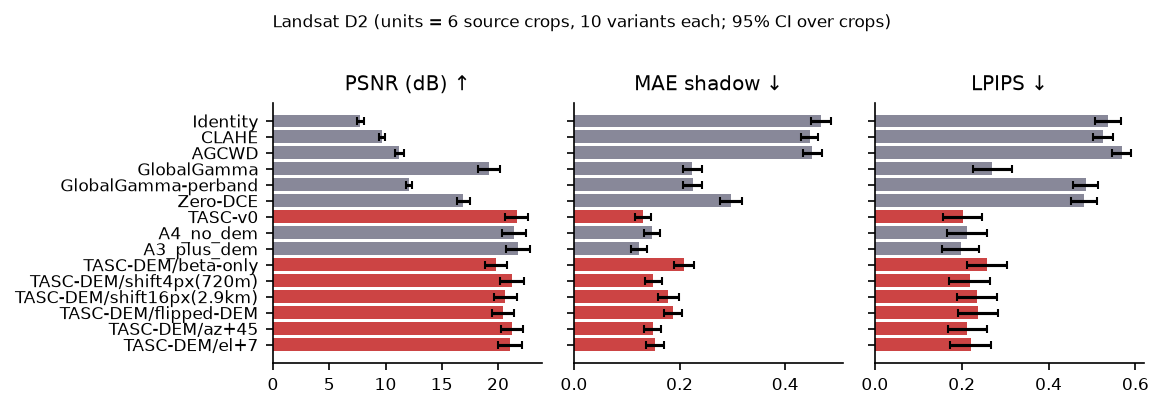
\includegraphics[width=0.8\columnwidth]{../figures/fig_d2_methods.png}
\caption{Landsat D2: PSNR, shadow MAE and LPIPS for selected methods and controls (bars: 95 \% bootstrap CI over the six source crops; TASC variants in red).}
\label{fig:d2}
\end{figure}
\subsection{Integrity controls and ablations on D2}
Table~\ref{tab:d2abl} lists controls (crop-level n = 6 for all intervals). Replacing the shadow term with a constant weight ($\beta$-only) loses 1.86 dB (CI 1.42--2.22), a flipped DEM loses 1.20 dB, and shifting the DEM by 720 m and 2.9 km loses 0.40 and 1.0 dB, so the benefit depends on correctly registered terrain. Azimuth errors of $\pm$15$^{\circ}$ cost about 0.05 dB and +45$^{\circ}$ costs 0.42 dB. Two controls expose the limits of the metric. First, a sun elevation 7$^{\circ}$ \emph{below} the metadata gives \textbf{higher} PSNR (22.45 dB) than the true elevation: a larger shadow field lifts under-exposed images more, so PSNR is not a measure of geometric correctness. Second, removing the DCT detail step is marginally \emph{better} on PSNR (+0.12 dB, CI 0.10--0.14) and shadow MAE (0.124 versus 0.130), so the detail step is not supported on this benchmark. Applying the gamma per band instead of through the shared gain loses 6.40 dB and raises the NDVI error from 0.018 to 0.162. The block-smoothing steps (hard blocks versus smoothed field) differ by under 0.02 dB.

\begin{table}[t]
\caption{D2 controls and ablations (means over 60 pairs; the table reports pair-level means, intervals are in \texttt{tables/d2\_vs\_tascv0.csv}).}
\label{tab:d2abl}
\centering\scriptsize
\setlength{\tabcolsep}{2.5pt}
\resizebox{\columnwidth}{!}{%
\begin{tabular}{lcc}
\toprule
Variant & PSNR & MAE shadow \\
\midrule
TASC-v0 (true DEM and sun) & 21.65 & 0.130 \\
image-only (no DEM) & 21.43 & 0.148 \\
$\beta$-only (constant weight) & 19.79 & 0.209 \\
flipped DEM & 20.45 & 0.187 \\
DEM shifted 720 m & 21.25 & 0.150 \\
DEM shifted 2.9 km & 20.65 & 0.179 \\
azimuth +15$^{\circ}$ / $-$15$^{\circ}$ / +45$^{\circ}$ & 21.59 / 21.58 / 21.23 & 0.132 / 0.133 / 0.149 \\
elevation +7$^{\circ}$ / $-$7$^{\circ}$ & 21.07 / 22.45 & 0.153 / 0.102 \\
no DCT detail step & 21.77 & 0.124 \\
global gamma + DCT (A0) & 20.27 & 0.209 \\
per-band gamma (A5) & 15.25 & 0.131 \\
\bottomrule
\end{tabular}}
\end{table}
\subsection{Real terrain: Sentinel-2 and Copernicus DEM}
Sentinel-2 has no ground-truth illumination. The statistical unit is the region (tiles averaged to scenes, scenes to regions): 4 development regions and 2 held-out regions, so every Sentinel-2 statement below is \textbf{exploratory}, and no Wilcoxon p-values exist for n < 5. All shadow masks are derived from the Copernicus DEM, the same source that drives TASC-DEM; metrics that use them favour DEM-aware methods (circularity).

\textbf{Spectral preservation (corrected metric).} Spectral angle, NDVI/NDWI error and band-ratio deviation of the output relative to the \emph{input} are exactly zero (to floating-point rounding) for every shared-gain method --- TASC image-only, TASC-DEM and their ablations, global gamma, CLAHE+shared and AGCWD+shared --- in both the development and held-out regions, because these methods multiply all bands of a pixel by one factor. This is a property of the construction and not an empirical advantage over the input: the input compared with itself also gives 0$^{\circ}$, the metrics cannot discriminate among shared-gain methods, and band-ratio preservation is not recovery of surface reflectance (the input's own atmospheric and sensor effects are preserved). Methods that do not share the gain change the spectra: per-band global gamma 10.3$^{\circ}$ (development) and 7.0$^{\circ}$ (held out), CLAHE 6.8$^{\circ}$ and 6.8$^{\circ}$, AGC 11.7$^{\circ}$ and 5.8$^{\circ}$, AGCWD 4.2$^{\circ}$ and 3.9$^{\circ}$, HE 12.7$^{\circ}$ and 10.1$^{\circ}$, the per-band TASC variants 13.8$^{\circ}$ (DEM-assisted) and 19.2$^{\circ}$ (image-only) in the development regions, the topographic corrections 2.4--2.5$^{\circ}$ and 4.4$^{\circ}$, and Zero-DCE 2.1$^{\circ}$ and 2.3$^{\circ}$ (NDVI error 0.025 and 0.027; NDWI error 0.025 and 0.009). These values are conditional on the pixels used: clipped (zero) reflectances and vectors with norm below 0.01 are excluded (about 10 \% of valid pixels in the development regions and 8 \% in the held-out regions for the input; 21 \% and 19 \% for Zero-DCE, and 22 \% and 21 \% for AGCWD+shared, whose outputs fall below the norm threshold); counts are in \texttt{tables/s2\_sam\_exclusions.csv}, and a threshold of 0.03 gives the same ordering. \emph{An earlier version of this paper reported TASC at 8.2$^{\circ}$ against 8.9$^{\circ}$ for the input; that comparison came from a defective metric and is withdrawn} (Section VIII and \texttt{reports/scientific\_corrections.md}).

On the development regions (n = 4) the DEM-assisted variant lifts terrain shadows by 0.218 versus 0.193 for image-only (difference 0.025, CI $-$0.003 to 0.054), and its lift is more selective (dark-lit/shadow ratio 0.29 versus 0.44). Among the methods that preserve spectra, TASC-DEM (true sun angles) has the largest shadow lift; AGC (0.212) and HE (0.193) lift similarly but clip 50--60 \% of bright pixels, and the per-band variants (TASC-DEM per band 0.331, TASC-image per band 0.302) lift more but change the spectra substantially. Over all six regions the shadow-lift difference between TASC-DEM and image-only is 0.034 (CI 0.011--0.056), but Holm-corrected p-values are 0.84--1.00. The controls behave as expected on this circular proxy: a wrong DEM or a DEM shifted by 1 km reduces the shadow lift (0.169 and 0.184) and the selectivity falls back to the image-only level (0.44 and 0.43), and a constant weight ($\beta$-only) gives the smallest lift (0.150). In the two held-out regions (sun elevation 7--20$^{\circ}$) the DEM variant again has the largest shadow lift among spectra-preserving methods (0.156 versus 0.105 image-only, wrong DEM 0.113), but the selectivity ratio is unstable (0.41 versus 1.37).

The material-matched check does \textbf{not} support a general equalisation benefit: vegetation in shadow versus lit becomes closer in brightness under image-only TASC (equalisation gain 0.197), global gamma (0.320), per-band global gamma (0.586) and CLAHE (0.623) than under TASC-DEM (0.012); in the held-out regions TASC-DEM is $-$0.433 and image-only $-$0.315. Part of the reason is that this metric rewards methods that brighten shadows regardless of terrain and uses a DEM-derived mask; with few vegetated shadow pixels in winter Alpine, Rocky and Atacama scenes it is also noisy. Topographic corrections C and SCS+C change little (shadow lift $-$0.007 and $-$0.006).

\begin{table}[t]
\caption{Sentinel-2 (mean over regions). Lift is the mean luminance gain in DEM-shadow pixels. SAM is the corrected spectral angle between output and input (preservation, not accuracy). Dev = 4 development regions, HO = 2 held-out regions.}
\label{tab:s2}
\centering\scriptsize
\setlength{\tabcolsep}{2.5pt}
\resizebox{\columnwidth}{!}{%
\begin{tabular}{lccccc}
\toprule
Method & Lift dev & Lift HO & NDVI err dev & SAM dev ($^{\circ}$) & SAM HO ($^{\circ}$) \\
\midrule
Identity & 0.000 & 0.000 & 0.000 & 0.00 & 0.00 \\
Global gamma & 0.126 & 0.065 & 0.000 & 0.00 & 0.00 \\
Global gamma, per band & 0.127 & 0.080 & 0.118 & 10.33 & 7.01 \\
CLAHE & 0.056 & 0.024 & 0.075 & 6.78 & 6.84 \\
AGC & 0.212 & 0.089 & 0.130 & 11.72 & 5.80 \\
AGCWD & 0.119 & 0.110 & 0.052 & 4.17 & 3.91 \\
HE & 0.193 & 0.013 & 0.136 & 12.72 & 10.11 \\
Zero-DCE & 0.124 & 0.116 & 0.025 & 2.13 & 2.34 \\
C-correction & -0.007 & 0.016 & 0.025 & 2.52 & 4.45 \\
SCS+C & -0.006 & 0.013 & 0.024 & 2.39 & 4.41 \\
TASC image-only & 0.193 & 0.105 & 0.000 & 0.00 & 0.00 \\
TASC-DEM & 0.218 & 0.156 & 0.000 & 0.00 & 0.00 \\
TASC-DEM, wrong DEM & 0.169 & 0.113 & 0.000 & 0.00 & 0.00 \\
TASC-DEM, shift 1 km & 0.184 & 0.132 & 0.000 & 0.00 & 0.00 \\
TASC-DEM, $\beta$-only & 0.150 & 0.076 & 0.000 & 0.00 & 0.00 \\
TASC-DEM, per band & 0.331 & 0.299 & 0.150 & 13.81 & 11.00 \\
\bottomrule
\end{tabular}}
\end{table}
\begin{figure}[t]
\centering
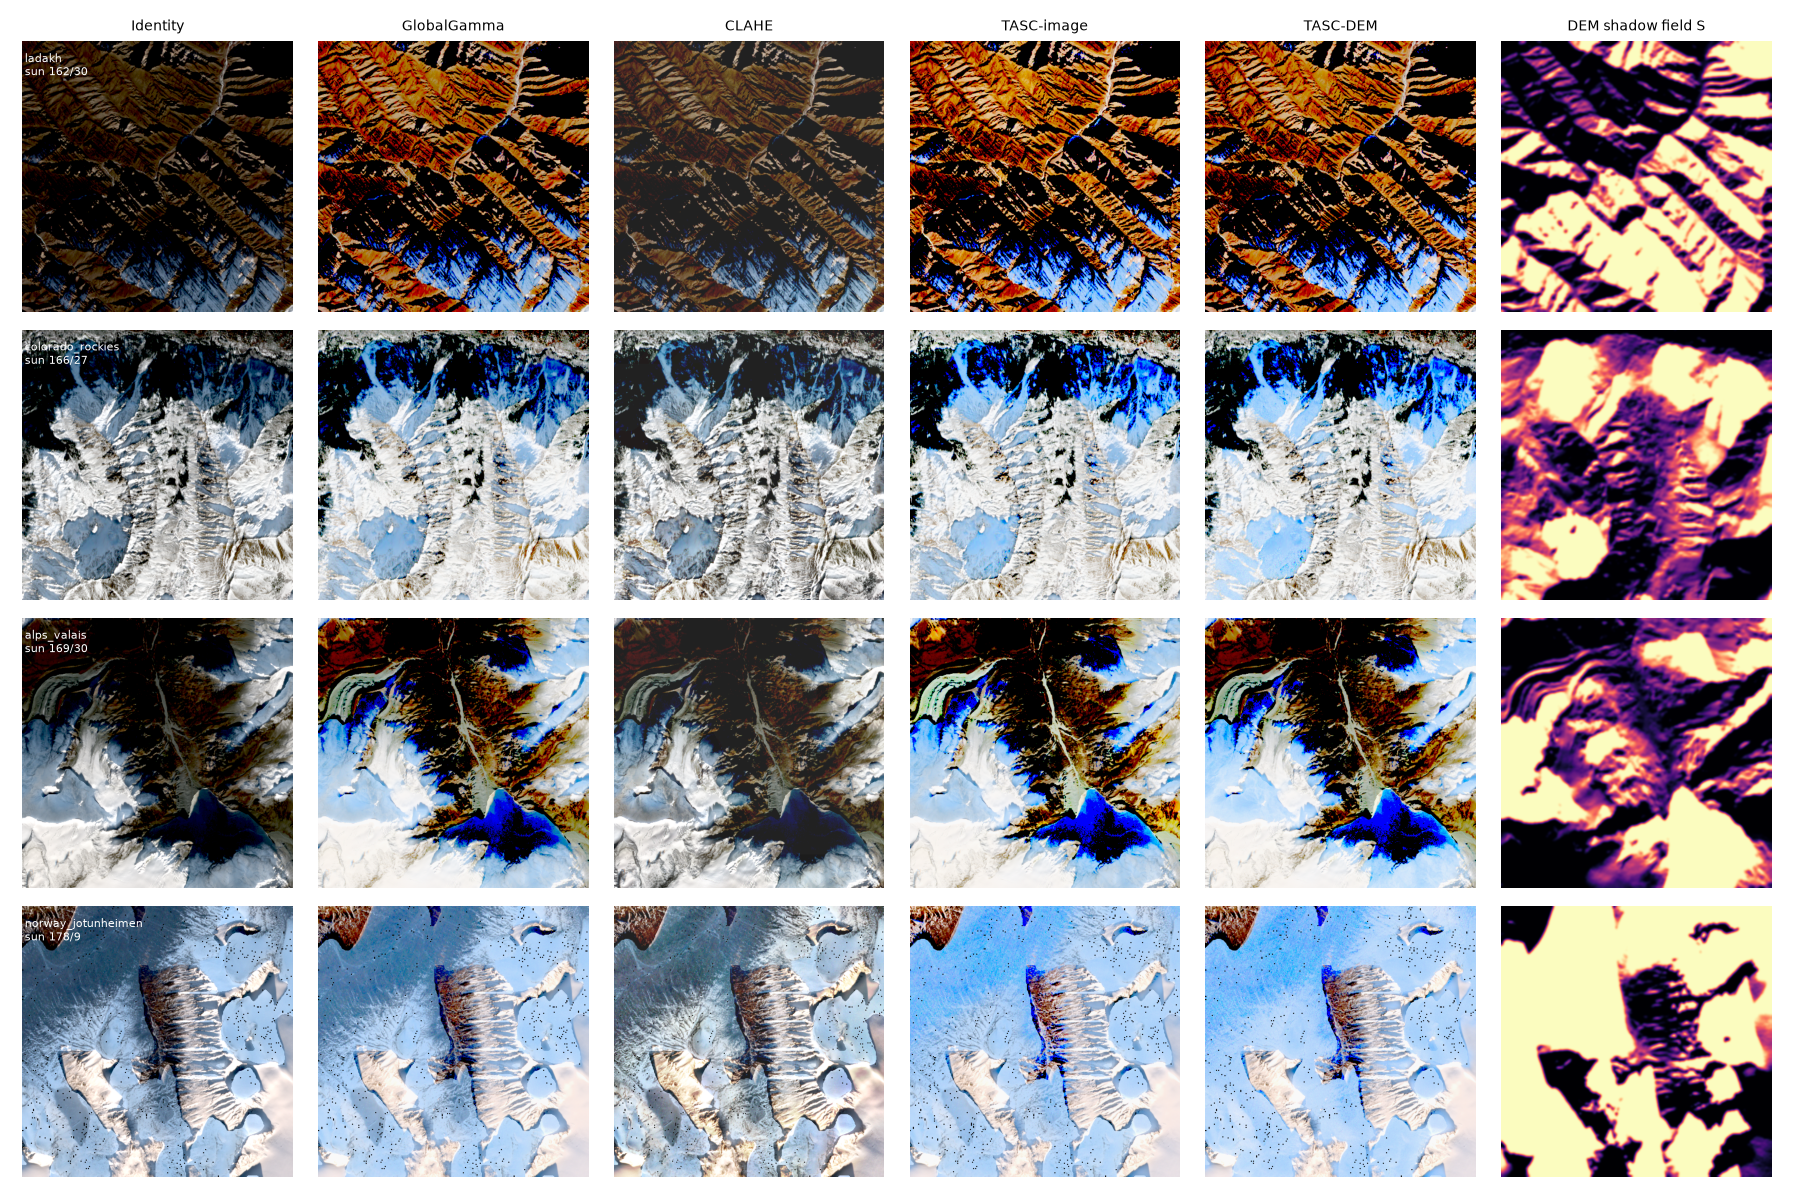
\includegraphics[width=0.95\columnwidth]{../figures/fig_qual_s2.png}
\caption{Qualitative Sentinel-2 examples: input, global gamma, CLAHE, TASC image-only, TASC-DEM, and the DEM shadow field S (rows: Ladakh, Colorado Rockies, Alps Valais: development; Jotunheimen: held out). Display gamma 1/2.2 is applied for viewing only. The two TASC variants are visually very similar; shadows are lifted but keep their blue cast because the shared gain preserves band ratios.}
\label{fig:qual}
\end{figure}
\subsection{Synthetic low light: AID and iSAID-dark}
On AID (Table~\ref{tab:aid}) the image-only method is \textbf{not competitive} against full-reference metrics. The best baseline on every full-reference metric is per-band global gamma (PSNR 17.51 dB, SSIM 0.490, LPIPS 0.555), followed by Zero-DCE (16.46 dB, 0.420, 0.575). TASC-image improves over the unprocessed input in PSNR (11.51 versus 10.32 dB; +1.19 dB, CI 0.64--1.73), but it is 4.15 dB below global gamma (CI $-$4.53 to $-$3.78), 4.94 dB below Zero-DCE ($-$5.40 to $-$4.51), 5.99 dB below per-band global gamma ($-$6.49 to $-$5.52) and 2.15 dB below CLAHE, and its SSIM (0.211) and LPIPS (0.763) are worse than the input (0.256 and 0.594). Among the spectra-preserving (shared-gain) methods TASC-image has the lowest noise amplification (0.50; per-band variants reach 0.40) and no new clipped highlights. The three degradations of a source image are averaged before testing (210 independent source images). The ablation points to the global exposure step: removing it gives 15.56 dB, matching global gamma (15.66 dB), while a global-only variant reaches 12.08 dB. Per degradation, TASC-image is above the input in PSNR for all three (non-uniform 13.18 versus 12.30 dB, uniform 12.50 versus 10.27 dB, severe 8.85 versus 8.39 dB), but its SSIM is below the input for all three, and in the severe case all methods struggle (best 12.4 dB, per-band global gamma). A plausible explanation, supported by this ablation but not isolated in a dedicated experiment, is that the fixed target $\tau$ = 0.55 over-brightens synthetic images whose originals have lower mean intensity, which full-reference metrics penalise.

On iSAID-dark, the units are parent images (46: the crops of the validation split and the three darkness levels of each high-pixel scene are averaged per parent), not the 138 files. TASC-image has PSNR 9.51 dB, below the unprocessed input (11.78 dB; $-$2.26 dB, CI $-$3.19 to $-$1.36), below global gamma (11.13 dB) and 3.87 dB below Zero-DCE (13.38 dB; CI $-$4.21 to $-$3.54) and 4.89 dB below the best baseline, per-band global gamma (14.40 dB; CI $-$5.12 to $-$4.64).

\begin{table}[t]
\caption{AID synthetic low light (210 source images, three degradations averaged within image).}
\label{tab:aid}
\centering\scriptsize
\setlength{\tabcolsep}{2.5pt}
\resizebox{\columnwidth}{!}{%
\begin{tabular}{lcccccc}
\toprule
Method & PSNR & SSIM & LPIPS & New clipped bright & Halo & Noise amp. \\
\midrule
Identity & 10.32 & 0.256 & 0.594 & 0.000 & 0.000 & 1.00 \\
HE & 12.13 & 0.293 & 0.751 & 0.483 & 0.012 & 1.03 \\
CLAHE & 13.66 & 0.376 & 0.594 & 0.001 & 0.001 & 1.05 \\
AGC & 12.26 & 0.305 & 0.733 & 0.502 & 0.023 & 1.12 \\
AGCWD & 13.87 & 0.328 & 0.630 & 0.114 & 0.002 & 1.21 \\
Global gamma & 15.66 & 0.308 & 0.659 & 0.000 & 0.002 & 0.52 \\
Global gamma, per band & 17.51 & 0.490 & 0.555 & 0.000 & 0.004 & 0.56 \\
Zero-DCE & 16.46 & 0.420 & 0.575 & 0.000 & 0.001 & 0.86 \\
2D-gamma & 9.76 & 0.264 & 0.650 & 0.000 & 0.005 & 1.10 \\
TASC-image & 11.51 & 0.211 & 0.763 & 0.000 & 0.027 & 0.50 \\
TASC-image, no global exposure & 15.56 & 0.317 & 0.651 & 0.000 & 0.001 & 0.56 \\
TASC-image, per band & 14.31 & 0.439 & 0.613 & 0.001 & 0.013 & 0.40 \\
\bottomrule
\end{tabular}}
\end{table}
\begin{table}[t]
\caption{iSAID-dark (46 parent images; crops and darkness levels averaged within parent). LPIPS is omitted: its values for the 1080p images are about 1 for all methods and not discriminative.}
\label{tab:isaid}
\centering\scriptsize
\setlength{\tabcolsep}{2.5pt}
\resizebox{\columnwidth}{!}{%
\begin{tabular}{lcccc}
\toprule
Method & PSNR & SSIM & Halo & Noise amp. \\
\midrule
Identity & 11.78 & 0.201 & 0.000 & 1.00 \\
HE & 11.19 & 0.149 & 0.027 & 1.05 \\
CLAHE & 12.96 & 0.176 & 0.008 & 1.03 \\
AGC & 12.19 & 0.169 & 0.037 & 0.90 \\
AGCWD & 12.53 & 0.168 & 0.010 & 1.10 \\
Global gamma & 11.13 & 0.112 & 0.033 & 0.60 \\
Global gamma, per band & 14.40 & 0.208 & 0.058 & 0.67 \\
Zero-DCE & 13.38 & 0.185 & 0.021 & 0.88 \\
2D-gamma & 11.05 & 0.185 & 0.004 & 1.07 \\
TASC-image & 9.51 & 0.098 & 0.117 & 0.65 \\
\bottomrule
\end{tabular}}
\end{table}
\begin{figure}[t]
\centering
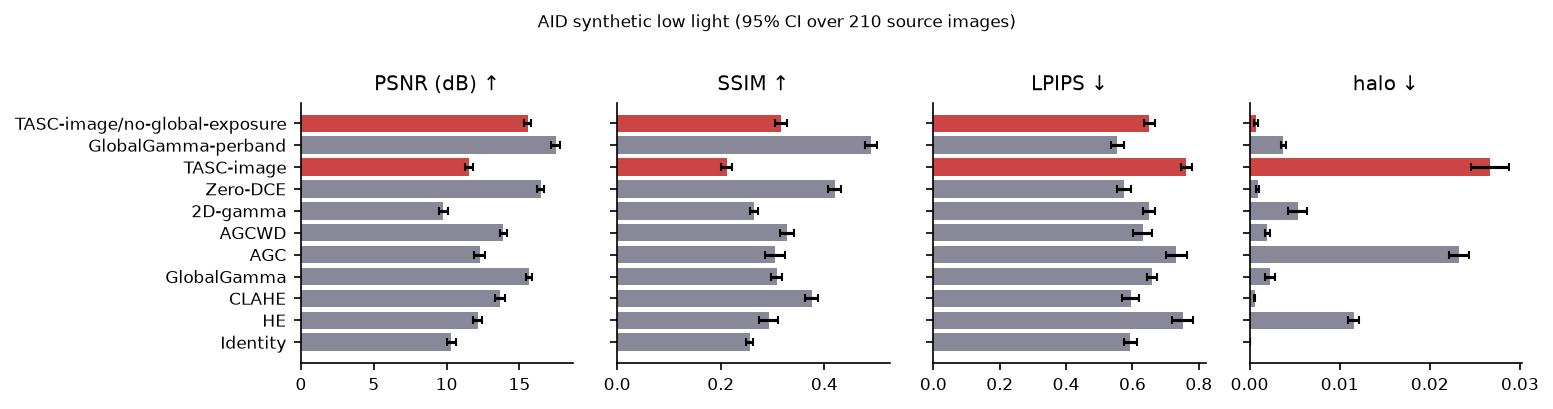
\includegraphics[width=0.8\columnwidth]{../figures/fig_aid_methods.png}
\caption{AID synthetic low light: PSNR, SSIM, LPIPS and halo rate (95 \% bootstrap CI over 210 source images; TASC-image in red). Bars are drawn from \texttt{tables/aid\_summary\_raw.csv} and include per-band global gamma (the best baseline) and the no-global-exposure ablation.}
\label{fig:aid}
\end{figure}
\subsection{Real low light: DarkRS and ExDark (no reference)}
Table~\ref{tab:darkrs} and Table~\ref{tab:exdark} report no-reference metrics on real night images. TASC-image brightens strongly but has low entropy on DarkRS (6.06 versus 6.48 input; $-$0.42, CI $-$0.47 to $-$0.37; only 2D-gamma is lower, 5.71) and the lowest EME (2.76 versus 7.56 for the input), and its BRISQUE is worse than the input (24.5 versus 18.3; +6.1, CI 4.8--7.5). NIQE is indistinguishable from the input on DarkRS (9.24 versus 9.12, $p_{\mathrm{Holm}}$ = 0.046, CI $-$0.01 to 0.23) and slightly better on ExDark (11.71 versus 12.27; $-$0.56, CI $-$0.80 to $-$0.31), where BRISQUE is again worse (29.1 versus 23.9). On ExDark, AGCWD attains the best BRISQUE (20.4) and HE the best NIQE (10.97). TASC-image has the lowest noise amplification on DarkRS (0.43) but not on ExDark (0.78; global gamma 0.69), and its low EME and entropy mean that low noise amplification is partly the effect of a flatter output rather than purely cleaner output. We find no support for contrast improvement from the image-only method on real night images with these metrics; the metrics are imperfect and no human study was done.

\begin{table}[t]
\caption{DarkRS, real night images, no reference (n = 86).}
\label{tab:darkrs}
\centering\scriptsize
\setlength{\tabcolsep}{2.5pt}
\resizebox{\columnwidth}{!}{%
\begin{tabular}{lccccc}
\toprule
Method & Entropy & EME & BRISQUE & NIQE & Noise amp. \\
\midrule
Identity & 6.48 & 7.56 & 18.3 & 9.12 & 1.00 \\
HE & 7.39 & 11.02 & 32.5 & 8.84 & 1.21 \\
CLAHE & 7.14 & 9.96 & 29.3 & 9.41 & 1.32 \\
AGC & 7.20 & 7.41 & 27.7 & 9.09 & 0.91 \\
AGCWD & 7.19 & 9.19 & 26.4 & 9.37 & 1.10 \\
Global gamma & 6.75 & 3.61 & 21.9 & 9.14 & 0.54 \\
Global gamma, per band & 6.80 & 3.57 & 22.2 & 9.10 & 0.55 \\
Zero-DCE & 7.05 & 5.93 & 33.4 & 9.43 & 0.89 \\
2D-gamma & 5.71 & 6.83 & 20.8 & 8.87 & 1.16 \\
TASC-image & 6.06 & 2.76 & 24.5 & 9.24 & 0.43 \\
\bottomrule
\end{tabular}}
\end{table}
\begin{table}[t]
\caption{ExDark, real low-light images, no reference (400 of 7,363 images).}
\label{tab:exdark}
\centering\scriptsize
\setlength{\tabcolsep}{2.5pt}
\resizebox{\columnwidth}{!}{%
\begin{tabular}{lccccc}
\toprule
Method & Entropy & EME & BRISQUE & NIQE & Noise amp. \\
\midrule
Identity & 5.80 & 9.04 & 23.9 & 12.26 & 1.00 \\
HE & 6.91 & 11.29 & 32.8 & 10.97 & 1.36 \\
CLAHE & 6.49 & 9.27 & 24.2 & 12.17 & 1.31 \\
AGC & 6.77 & 11.22 & 25.5 & 11.46 & 1.10 \\
AGCWD & 6.58 & 10.96 & 20.4 & 11.71 & 1.14 \\
Global gamma & 6.34 & 6.75 & 23.8 & 12.08 & 0.69 \\
Global gamma, per band & 6.46 & 5.77 & 27.4 & 11.80 & 0.76 \\
Zero-DCE & 6.67 & 9.42 & 26.1 & 12.19 & 1.00 \\
2D-gamma & 5.45 & 9.19 & 25.2 & 11.61 & 1.54 \\
TASC-image & 5.88 & 6.66 & 29.1 & 11.71 & 0.78 \\
\bottomrule
\end{tabular}}
\end{table}
\subsection{Downstream: AID scene classification probe (E7)}
A frozen-feature linear probe reaches 0.881 accuracy on clean test images. Each degradation is analysed separately over the same 210 test images (the three degradations of one image are never pooled as independent samples). After degradation, accuracy for the unprocessed input is 0.838 (uniform), 0.857 (non-uniform) and 0.581 (severe). TASC-image lowers accuracy to 0.638, 0.710 and 0.343, i.e. $-$0.200 (CI $-$0.271 to $-$0.133), $-$0.148 ($-$0.214 to $-$0.081) and $-$0.238 ($-$0.314 to $-$0.167) relative to the input; all intervals exclude zero. The other methods stay within about $\pm$0.06 of the input; the only nominal gains are AGCWD (+0.043, CI 0.005--0.081) and Zero-DCE (+0.043, CI $-$0.005 to 0.090) under the severe degradation, without correction for multiple comparisons. Per-band global gamma, the strongest full-reference baseline, is also within this range (0.824, 0.852, 0.610). No method recovers clean accuracy under the severe degradation. Enhancement therefore does not help this probe, and the image-only method harms it. Detection and segmentation were not run.

\begin{table}[t]
\caption{Linear-probe accuracy on 210 AID test images.}
\label{tab:e7}
\centering\scriptsize
\setlength{\tabcolsep}{2.5pt}
\resizebox{\columnwidth}{!}{%
\begin{tabular}{lccc}
\toprule
Method & Uniform & Non-uniform & Severe \\
\midrule
Clean reference & 0.881 & 0.881 & 0.881 \\
Identity & 0.838 & 0.857 & 0.581 \\
Global gamma & 0.810 & 0.805 & 0.524 \\
Global gamma, per band & 0.824 & 0.852 & 0.610 \\
CLAHE & 0.829 & 0.852 & 0.605 \\
AGCWD & 0.824 & 0.852 & 0.624 \\
HE & 0.814 & 0.795 & 0.595 \\
Zero-DCE & 0.857 & 0.833 & 0.624 \\
TASC-image & 0.638 & 0.710 & 0.343 \\
\bottomrule
\end{tabular}}
\end{table}
\subsection{Efficiency}
On a single CPU process (1 MP image, four threads), TASC-image takes about 114 ms/MP, versus 13 ms/MP for CLAHE, 21 ms/MP for HE, 22 ms/MP for AGCWD, 51 ms/MP for global gamma and about 33 s/MP for Zero-DCE on CPU (a GPU would change this ranking; none was used). The DEM-assisted variant was not timed separately: the ray-marched shadow field adds a cost that scales with relief and window size. Peak memory was not reliably measured (Section VIII).

\section{Statistical Analysis}
Independent units: source crops for D2 (n = 6, ten dependent variants averaged within crop, all from one Landsat scene), source images for AID (210; the three degradations averaged within image) and for E7 (each degradation analysed separately), parent images for iSAID-dark (46), images for DarkRS (86) and ExDark (400; images from the same photographic series cannot be excluded), and regions for Sentinel-2 (4 development, 2 held out, 6 pooled). Intervals are percentile bootstrap intervals over these units; Wilcoxon tests are only computed for n $\geq$ 5 and corrected with Holm within each (reference, metric) family. With six D2 crops the smallest attainable p-value is 0.031, so no D2 comparison survives correction; for Sentinel-2 no test is available for 4 or 2 regions and the six-region Holm-corrected p-values are 0.84--1.00. Where tests are possible with larger n (AID, iSAID-dark, DarkRS, ExDark, E7), the large differences reported above are far beyond Holm-corrected significance; the notable non-significant findings are NIQE on DarkRS and ExDark against several baselines, and entropy on ExDark against the input ($p_{\mathrm{Holm}}$ = 0.092).

\section{Discussion}
\emph{What the experiments support.} (i) On the controlled terrain-shading benchmark, a training-free, shared-gain, locally adaptive gamma outperforms the baselines we tested, in every one of six crops, though not at a formally significant level. (ii) The DEM is used: the controls show degradation for wrong, flipped and shifted terrain. (iii) Shared-gain methods leave the spectral angle to the input at zero on D2 and keep NDVI unchanged; this is preservation of the input's band ratios, which is not the same as recovering surface reflectance, and the recovered image inherits whatever spectral error the degraded input has. (iv) On real Sentinel-2 scenes with real sun angles, the DEM-assisted variant lifts terrain shadow more than the image-only variant (about +0.03 luminance units, exploratory, circular mask).

\emph{What they do not support.} (i) The DEM benefit on D2 depends on the unit of analysis and is built into that benchmark. (ii) We found no evidence that DEM-aided TASC equalises same-material brightness across shadow better than simpler methods. (iii) The image-only method is not a competitive general low-light enhancer: it is below per-band global gamma, Zero-DCE, global gamma and CLAHE on synthetic low light, below the unprocessed input on iSAID-dark, worse than the input on BRISQUE for real night images, and harmful for a classification probe. (iv) The DCT detail step has no measured benefit on D2.

\emph{Visual behaviour.} In the qualitative examples (Fig.~\ref{fig:qual}) TASC lifts terrain shadows more than CLAHE and similarly to global gamma, but shadowed snow keeps its blue cast by construction (ratios are preserved), and the image-only and DEM-assisted outputs are hard to tell apart by eye; the measured differences are small.

\emph{Why.} The ablation on AID (removing the global exposure step gives +4.0 dB and recovers global gamma's score) indicates that the fixed target mid-level, tuned on D2, is the dominant factor for synthetic low light; we did not tune it, since the method was frozen. This is a hypothesis for future work, not a result. A related caution is that full-reference metrics on synthetic darkening favour methods that invert the darkening model.

\emph{Relation to prior work.} Spatially adaptive gamma correction for remote-sensing images (SAGC, SAMSIE) and topographic correction are established; this study evaluates one terrain-aware, spectrally consistent variant and does not claim novelty for these ideas. SAGC, SAMSIE and DFFN were not evaluated, so we make no comparative statement about them.

\emph{Recommendations (not implemented here, per the protocol).} Phase-4 candidates are an exposure-target calibration that is data-driven and region-aware, a re-examination of the detail step, and a Sentinel-2 evaluation against independently annotated shadows.

\section{Threats to Validity}
\emph{Circularity.} D2 shadows and Sentinel-2 shadow masks both derive from the same DEM that drives TASC-DEM. \emph{Few independent units.} D2 has six source crops from one scene; Sentinel-2 has six regions, two held out. \emph{Synthetic degradations.} AID and iSAID-dark are not real low light, and the references are the bright originals. \emph{Spectral metric.} The frozen \texttt{tasc.metrics.sam\_deg} was found to be defective (it reports 8.93$^{\circ}$ for identical Sentinel-2 input); all spectral-angle values in this paper come from a corrected metric (\texttt{research/trs/spectral.py}, \texttt{reports/scientific\_corrections.md}); clipped (zero) reflectance and vectors with norm below 0.01 are excluded and counted. \emph{Metrics.} NIQE, BRISQUE, EME and entropy are imperfect proxies, no user study was done, and LPIPS for 1080p iSAID images was not discriminative. \emph{Measurement.} Runtimes inside experiment stores were collected with four concurrent workers; only the single-process efficiency run is comparable. The peak-RSS values of the efficiency run are identical for all methods (4,397 MB), so memory is not reported. \emph{Baselines.} Re-implementations of AGC, AGCWD, HE, CLAHE and 2D gamma are not claimed to match published numbers. \emph{Elevation sensitivity.} PSNR rewards a mis-specified (lower) sun elevation on D2.

\section{Limitations and Missing Baselines}
SAGC \cite{huang2018sagc} and SAMSIE \cite{huang2022samsie} could not be evaluated because no verified official implementation was available; the labelled "2D-gamma" is an independent approximation and should not be read as either. The DFFN \cite{yao2024dffn} code and weights were downloaded and checksummed but were not executed: running downloaded third-party code was blocked by our sandbox policy and was not circumvented; DFFN is therefore reported as not evaluated. The downstream study covers classification only. The iSAID-dark version used is the one distributed with the DFFN repository (folder \texttt{iSAID2}) and was not matched to a published version number. The full limitation list is in the repository (\texttt{research/reports/limitations.md}).

\section{Conclusion}
A frozen training-free gamma method, evaluated across six datasets and a downstream probe with integrity controls, keeps the input's band ratios by construction and does well on the controlled terrain-shading task it was developed for, with evidence that correct terrain information matters; that evidence rests on six crops of a single scene and does not reach formal significance. Beyond that setting its advantage did not generalise: for synthetic and real low light and for a downstream probe, the image-only configuration was weaker than much simpler baselines, and the DEM benefit on real terrain is small, exploratory and statistically unresolved with six regions. These findings define the work needed before the method can be recommended outside controlled terrain shading.

\section*{Data and Code Availability}
Code, configurations, manifests, result tables and reports are in the repository on branch \texttt{research/illumination-aware-benchmark-v1}. Dataset files are not redistributed; checksums and acquisition scripts are provided. The reproduction command is \texttt{python research/scripts/run\_all\_research.py --config research/configs/research\_full.yaml --resume}.

\bibliographystyle{IEEEtran}
\bibliography{references}
\end{document}
